\section{Manifolds and Lie Groups}

Now we will give explicit defitions for manifolds, Lie groups, and Lie algebras.
There is a lot to talk about here and there is easily enough out there to fill an 
entire book so we will only talk about what is necessary in the context of geometry.

\subsection{Embedded Manifolds}
Before we explicitly define manifolds, we need to look at a simplified version which
we call \textit{embedded manifolds}. In a huge nutshell, a manifold is some kind
of space that looks like $\R^n$ locallly. Now we will explicitly define a manifold
and unpack the defition.

\begin{boxdef}{Manifold}{}
    Given two integers $N,m$ with $N \geq m \geq 1$, an $m$\textit{-dimensional smooth
    manifold in $\R^N$} (we will now just say ``manifold''), is a nonempty subset
    $M \subseteq \R^N$ such that for every point $p \in M$ there are two open subsets
    $\Omega \subseteq \R^m$ and $U \subseteq M$ with $p\in U$, and a smooth function
    $\varphi: \Omega \to \R^N$ such that $\varphi$ is a homeomorphism, $\varphi ' (t_0)$
    is injective, where $t_0 = \varphi^{-1}(p)$.
    \vspace{5mm}
    
    The function $\varphi: \Omega \to U$ is a \textit{local parameterization} of $M$
    at $p$. If $0_m \in \Omega$ and $\varphi(0_m) = p$, we say that $\varphi$ is
    \textit{centered} at $p$.
\end{boxdef}

Although the defition is lengthy, it is very precise and actually a little more intuitive
than it may initially seem. Also note that because $\varphi$ is a homeomorphism,
it admits a smooth inverse $\varphi^{-1}:U \to \Omega$ called a \textit{chart}. These
charts are what allow us to travel between $\R^n$ and a given manifold. The charts
tell us how to translate the language of the manifold onto the base field. Lets 
look at a pretty picture of a manifold in $\R^n$.

\begin{figure}[h]
\centering
\tikzset{every picture/.style={line width=0.75pt}} %set default line width to 0.75pt        
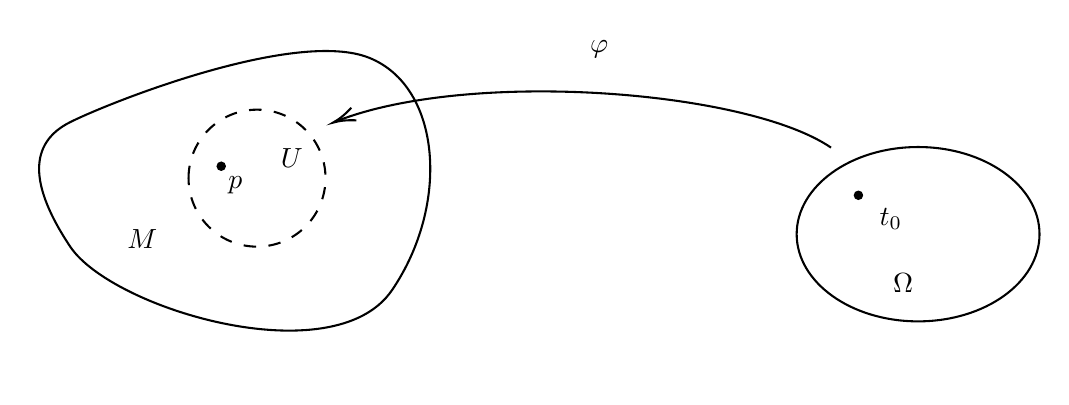
\begin{tikzpicture}[x=0.75pt,y=0.75pt,yscale=-1,xscale=1]
%uncomment if require: \path (0,310); %set diagram left start at 0, and has height of 310

%Shape: Polygon Curved [id:ds3188555190279363] 
\draw   (67,96) .. controls (87,86) and (176,51) .. (211,65) .. controls (246,79) and (250,136) .. (222,177) .. controls (194,218) and (87,186) .. (67,156) .. controls (47,126) and (47,106) .. (67,96) -- cycle ;
%Shape: Circle [id:dp22161905680813043] 
\draw  [dash pattern={on 4.5pt off 4.5pt}] (124,123) .. controls (124,104.77) and (138.77,90) .. (157,90) .. controls (175.23,90) and (190,104.77) .. (190,123) .. controls (190,141.23) and (175.23,156) .. (157,156) .. controls (138.77,156) and (124,141.23) .. (124,123) -- cycle ;
%Shape: Circle [id:dp5483624745402305] 
\draw  [fill={rgb, 255:red, 0; green, 0; blue, 0 }  ,fill opacity=1 ] (141.5,117.25) .. controls (141.5,116.28) and (140.72,115.5) .. (139.75,115.5) .. controls (138.78,115.5) and (138,116.28) .. (138,117.25) .. controls (138,118.22) and (138.78,119) .. (139.75,119) .. controls (140.72,119) and (141.5,118.22) .. (141.5,117.25) -- cycle ;
%Shape: Ellipse [id:dp3498820164689296] 
\draw   (417,150) .. controls (417,126.8) and (443.19,108) .. (475.5,108) .. controls (507.81,108) and (534,126.8) .. (534,150) .. controls (534,173.2) and (507.81,192) .. (475.5,192) .. controls (443.19,192) and (417,173.2) .. (417,150) -- cycle ;
%Shape: Circle [id:dp7735858738895589] 
\draw  [fill={rgb, 255:red, 0; green, 0; blue, 0 }  ,fill opacity=1 ] (448.5,131.25) .. controls (448.5,130.28) and (447.72,129.5) .. (446.75,129.5) .. controls (445.78,129.5) and (445,130.28) .. (445,131.25) .. controls (445,132.22) and (445.78,133) .. (446.75,133) .. controls (447.72,133) and (448.5,132.22) .. (448.5,131.25) -- cycle ;
%Curve Lines [id:da5307662779865321] 
\draw    (433.55,108.28) .. controls (392.75,80.42) and (257.91,70.38) .. (194.5,95.89) ;
\draw [shift={(193.55,96.28)}, rotate = 337.57] [color={rgb, 255:red, 0; green, 0; blue, 0 }  ][line width=0.75]    (10.93,-3.29) .. controls (6.95,-1.4) and (3.31,-0.3) .. (0,0) .. controls (3.31,0.3) and (6.95,1.4) .. (10.93,3.29)   ;

% Text Node
\draw (141.75,120.65) node [anchor=north west][inner sep=0.75pt]    {$p$};
% Text Node
\draw (167,107.4) node [anchor=north west][inner sep=0.75pt]    {$U$};
% Text Node
\draw (93,146.4) node [anchor=north west][inner sep=0.75pt]    {$M$};
% Text Node
\draw (448.75,132.9) node [anchor=north west][inner sep=0.75pt]    {$ \begin{array}{l}
t_{0}\\
\end{array}$};
% Text Node
\draw (462,167.4) node [anchor=north west][inner sep=0.75pt]    {$\Omega $};
% Text Node
\draw (316,55.4) node [anchor=north west][inner sep=0.75pt]    {$\varphi $};
\end{tikzpicture}
\caption{A manifold $M$ and a local parameterization $\varphi$.}\label{figLabel}
\end{figure}

This visualization is key and will be paramount to understanding how we do analysis
on manifolds. It is worth noting too that $M$ is a topological space and $U$ is a
subspace endowed with the subspace topology. Perhaps the most basic example of a
manifold would be the unit sphere $S^2$ embedded in $\R^3$. It is pretty easy to
check the conditions for a manifold but the arithmetic is a little tedious (stereographic
projections ew).

In fact, every open subset of $\R^n$ is a manifold in a somewhat trivial way. For 
the parameterization, we just choose the inclusion map and the rest is trivial.
A great example would be the Lie group $GL(n,\R)$. Of course it is a manifold by
definition but assuming no Lie group structure, we can still view $GL(n,\R)$ as an
open subset of $\R^{n^2}$ as its complement is closed; the set of invertible matrices
is the inverse image of the determinant funtion, which is continuous of course (this
is worth proving if you haven't already).

\begin{boxex}{$GL(n,\C)$ as a manifold}{}
    For every $A \in M_n(\C)$, construct an analogous $2n \times 2n$ real matrix
    such that every entry $a + ib$ in $A$ is replaced by the matrix
    \begin{equation*}
        \begin{bmatrix}
            a & -b\\
            b & a
        \end{bmatrix}
    \end{equation*}
    We can represent this map by
    \begin{align*}
        \Phi &: M_n(\C) \to M_{2n}(\R)\\ \\
        A & \mapsto \begin{bmatrix}
            a & -b\\
            b & a
        \end{bmatrix}
    \end{align*}
    This map is obviously a group isomorphism so we can view $GL(n,\C)$ as a subgroup
    of $GL(2n,\R)$ and as a manifold in $\R^{(2n)^2}$.
\end{boxex}

Now we have a decent understanding of some properties of manifolds and their charts.
Now, we will look at how to jump between manifolds and the inverse images of their
respective charts.

\begin{boxdef}{Transition Maps}{}
    Given an $m$-dimensional manifold $M$ in $\R^n$, for every $p \in M$ and any
    two parameterizations $\varphi_1: \Omega_1 \to U_1$ and $\varphi_2: \Omega_2
    \to U_2$ of $M$ at $p$, if $U_1 \cap U_2 \neq \varnothing$, the map $\varphi_2^{-1}
    \circ \varphi_1 : \varphi_1^{-1}(U_1 \cap U_2) \to \varphi_2^{-1}(U_1 \cap U_2)$
    is a smooth diffeomorphism. These maps are called \textit{transition maps}.     
\end{boxdef}

In a nutshell, if there is some overlap of the images of parameterizations, given
sufficient conditions, we can construct a transition map to take elements from the
first open subset $\Omega_1$, to another $\Omega_2$. Note that these are maps between
open subsets of $\R^n$ and NOT maps between manifolds (we will talk about that later).

In general, it can be difficult to prove a given space is a manifold in an explicit
manner, so we want to have alternate ways of characterizing and identifying manifolds.
This leads us to a great proposition that will be extremely useful.

\begin{boxprop}{}{}
    butthole
\end{boxprop}